\documentclass[graphics]{beamer}

\usepackage{graphicx}
\usepackage{verbatim}
\usepackage{wrapfig}
\useoutertheme{shadow}
%\usecolortheme{orchid}
\usecolortheme{seahorse}
\usepackage{tikzsymbols}
\usepackage{textcomp}
\usepackage{parskip}

% math commands
\newcommand{\be}{\begin{eqnarray}}
\newcommand{\ee}{\end{eqnarray}}
\newcommand{\beq}{\begin{equation}}
\newcommand{\eeq}{\end{equation}}
\def\simless{\mathbin{\lower 3pt\hbox
      {$\rlap{\raise 5pt\hbox{$\char'074$}}\mathchar"7218$}}}
\def\simgreat{\mathbin{\lower 3pt\hbox
      {$\rlap{\raise 5pt\hbox{$\char'076$}}\mathchar"7218$}}} %> or of order

% variables

\def\toonscale{0.45}
\def\mboxy#1{\mbox{\small #1}}


\begin{comment}
\AtBeginSection[]{
  \frame{
    \frametitle{Outline}
    \tableofcontents[currentsection]
  }
}
\end{comment}

\title{Helical (Parity Odd) Initial conditions
}
\subtitle{}
\author[U. Pen]{\textcolor{green}{Ue-Li Pen, ASIAA, CITA}
\\[8mm] 
}
\date{September 5, 2022}


\begin{document}

\frame{
\begin{picture}(320,250)
\put(-50,0){
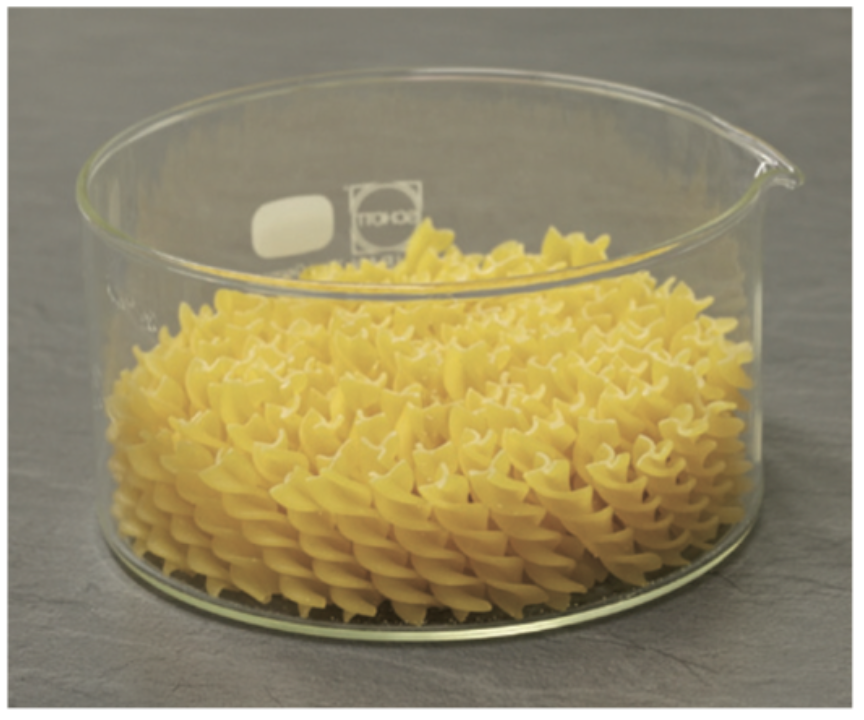
\includegraphics[width=5.5in]{Figures/helicalpasta.png}}
Schaller+12, Nature, 481, 261
\end{picture}
\vspace{-3in}
\titlepage
}

%\section*{Introduction}
\section{Helicity: Kitchen, sun, galaxy and beyond}

\begin{comment}
  \subsection{Outline}

  \frame{
    \frametitle{Outline}
    \tableofcontents
  }
\end{comment}

   \frame{
    \frametitle{Helicity}
    \begin{itemize}
        \item Macroscopic physics (gravity, E-M, etc) are parity symmetric
        \item
        \item recent claims of detection (Hou+22, Philcox 22), upper
          bounds (Motloch+22)
        \item large, abstract space of parity odd configurations in
          4PCF, difficult to quantify covariances and look-elsewhere effect
        \item quadric estimator classification
        \item includes galaxy spin
        \item generation mechanisms
     \end{itemize}
}

  \frame{
    \frametitle{Quadratic forms}
    \begin{itemize}
        \item analogy: CMB lensing
        \item deflection estimator: $d_i=T \partial_i \bar{T}$
          (Okamoto-Hu++03)
        \item shear estimator $\Gamma_{ij}=\partial_i T\partial_j T$
          (Zhu-ULP 2011.08251)
        \item 2 scalar ($\kappa,\gamma^E$), 1 pseudo scalar
          ($\gamma^B$) degree of freedom
          \item under lensing $\gamma^E=\kappa$ and $\gamma^B=0$
            \item $\gamma^B$ souced by multi-plane lensing
            \item $H=\gamma^E-\kappa$ sourced by tensor modes (Dodelson+02)
        \item lensing power is a 4PCF,  related to $g_{NL}$
        \item squeezed limit $L\ll l$ reduces 4PCF to E and B lensing
          power of $L$
        \item B power is parity-odd, not helical: excess power in B an
          indication of parity-odd  non-Gaussianity, distinct from
          helicity
\item 
     \end{itemize}
}
\frame{
    \frametitle{CMB}
\vspace{-0.15in}
\hspace{-0in}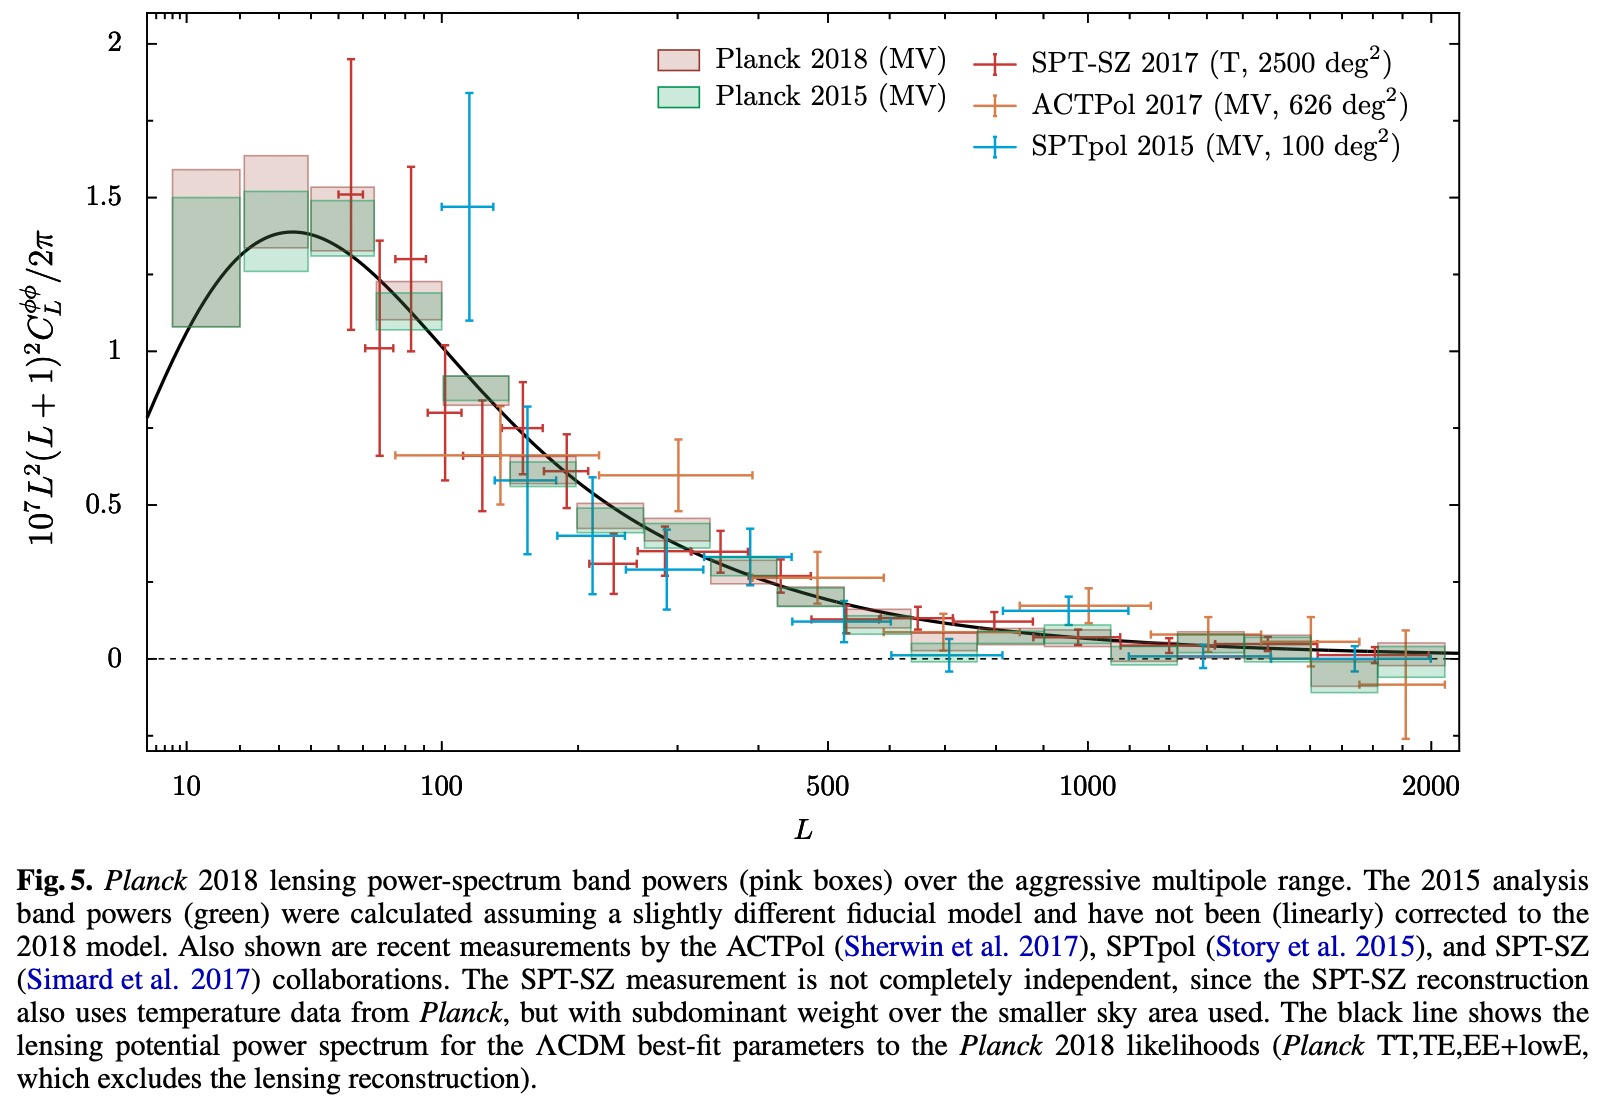
\includegraphics[width=4.2in]{Figures/plancklens.png}  

Planck 2018
  }

\frame{
    \frametitle{CMB-B}
\vspace{-0.15in}
\hspace{-0in}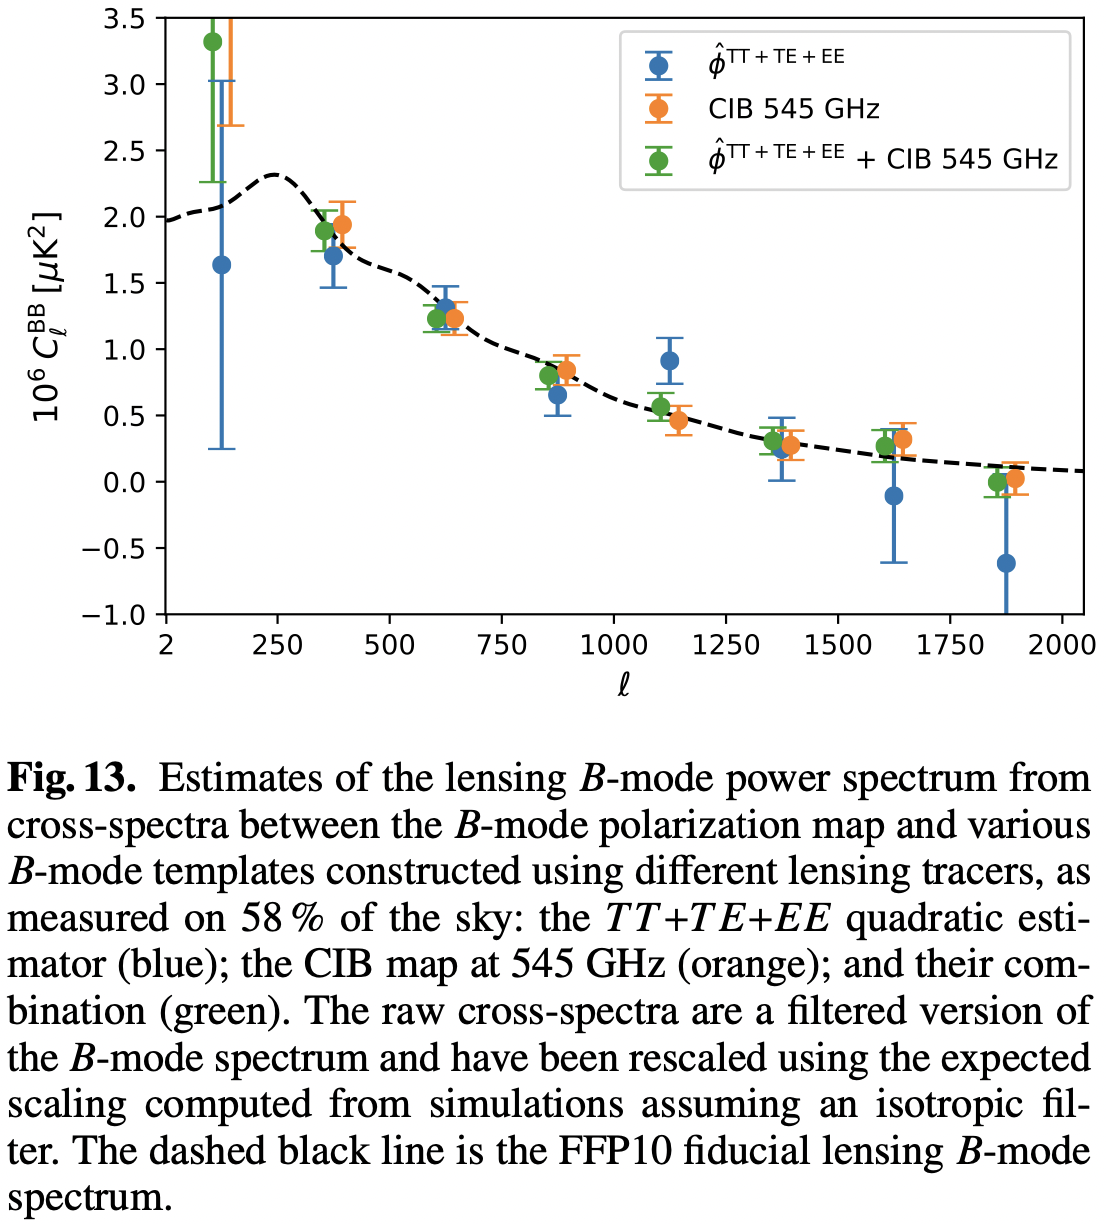
\includegraphics[width=2.8in]{Figures/plancklensb.png}  
Planck 2018
  }

  \frame{
%\vspace{-0.5in}
    \frametitle{3D quadratic form}
    \begin{itemize}
    \item Cosmic tides (ULP++2012, Masui++2010,Jeong++2012 )
    \item estimator $T_{ij}=\partial_i \bar{\delta} \partial_j
      \bar{\delta}$
    \item $T$ decomposed into 2 scalar, 2 vector, 2 tensor components
    \item scalar trace $t=T_{ii}$, longitudinal $l=\hat{k}_i\hat{k}_j (T-t\delta_{ij}/3)$
    \item vector and tensor projected onto left and right pseudoscalars
    \item $v^{L,R}=e^{L,R}_i \partial_j T_{ij}$, \ \ \ \ \ \  \  $h^{L,R}=e^{L,R}_i e^{L,R}_j T_{ij}$
    \item helical projection operator $e^{L,R}$: unit eigenvectors of curl operator
    \item Helical power asymmetry: $\eta=(P_L-P_R)/(P_L+P_R)$
    \item no analogy in CMB, requires 2 parity odd (helical) d.o.f
    \item vector $\eta<10^{-3}$ (Motloch+ 2022)
    \item 
    \end{itemize}
    }
      
\frame{
    \frametitle{Tidal scalars}
%\vspace{-0.5in}
\hspace{-0.6in}\includegraphics[width=4.8in]{Figures/tidesim.png}  

Zhu+ 22
  }


\frame{
    \frametitle{Data}
%\vspace{-0.5in}
\hspace{-0in}\includegraphics[width=2.9in]{Figures/tide.png}  
ULP+ 12
  }


  \frame{
%\vspace{-0.5in}
    \frametitle{Observables}
    \begin{itemize}
    \item 4PCF -- not intuitive due to large dimension, difficult to
      compute covariance (8PCF!)
    \item distinguish excess power in parity odd fields from helical
      power assymmetry!  Excess power is generic.
    \item galaxy spin
    \item magnetic field helicity
    \item Tidal:
    \item in analogy to B mode lensing map, create 4 helical
      pseudo-scalar maps
    \item vector, tensor helical auto and cross power for same helicity
    \item L-R cross correlation violated statistical isotropy
    \item 3 functions of $k$, huge reduction from 3-D function
    \end{itemize}
    }
       
  \frame{
%\vspace{-0.5in}
    \frametitle{Helicity kinematics}
    \begin{itemize}
    \item helical vector generically sources tensor quadratic
      helicity
      \item helical vector $B_j$ in quadratic form $T_{ij}=B_i B_j$
        fully helical, c.f. stress-energy sources for gravitational coupling
    \item quadratic vector helicity generation still open question
    \end{itemize}
    }
 
  \frame{
%\vspace{-0.5in}
    \frametitle{Helical sources}
    \begin{itemize}
    \item helical tensor modes (Jeong+12, Masui+17)
    \item Axion modes
    \item Lagrangian term $g\theta F \tilde{F}$
    \item modifies Maxwell equation $\dot{B}=\nabla\times E+g\dot{\theta}\nabla\times B$
    \item for coherent misalignment, leads to instability in single B
      helical mode
    \item proposed for early magnetogenesis (Campanelli++05)
    \item dark sector could lead to isocurvature scalar helicity conversion
    \end{itemize}
    }
      
  \frame{
    \frametitle{Galaxy Spin: Gas-DM simulations}
    \vspace{-0.1in}
    \center{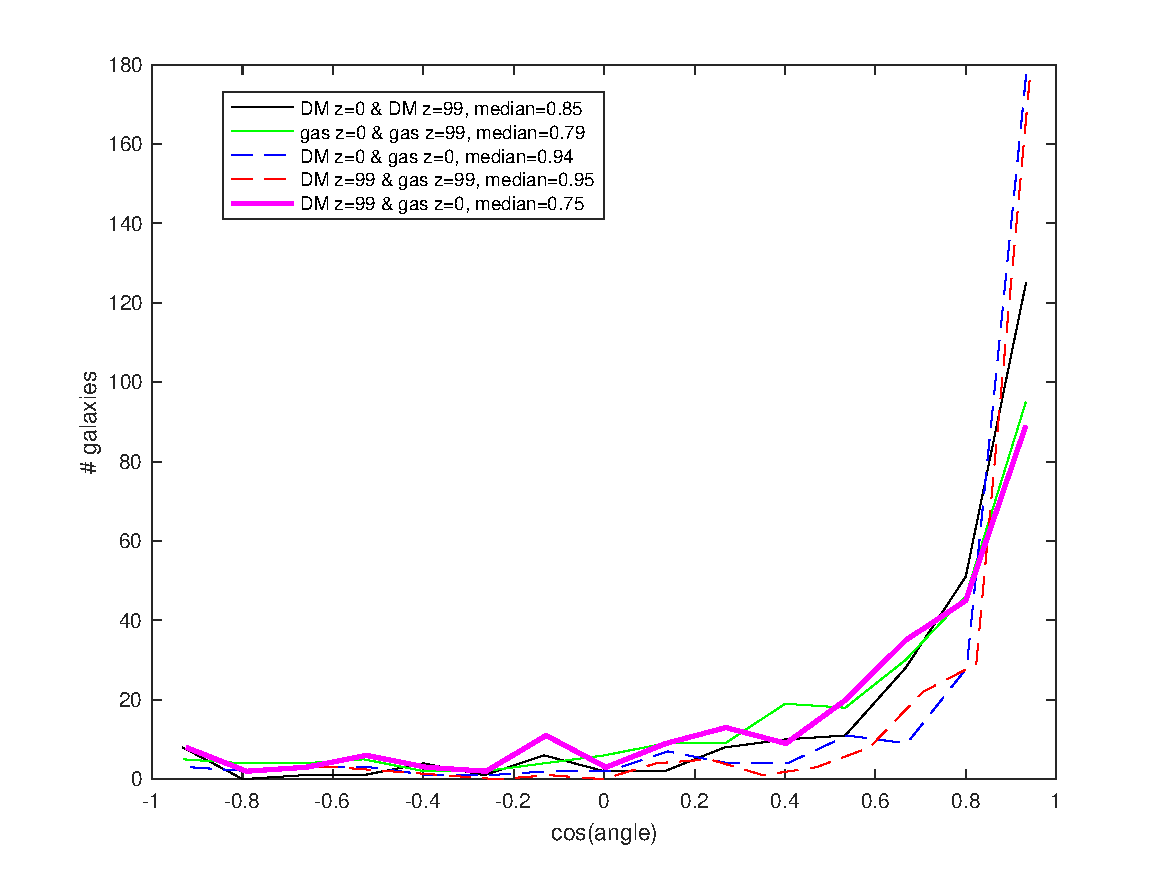
\includegraphics[width=4.01in]{Figures/Illustris_Lagrangian_AM_cosangle_distributions_allgas.pdf}}
    { Shy Genel, Illustris, private communication}
}


\frame{
    \frametitle{Measurement}
%\vspace{-0.5in}
\hspace{-0in}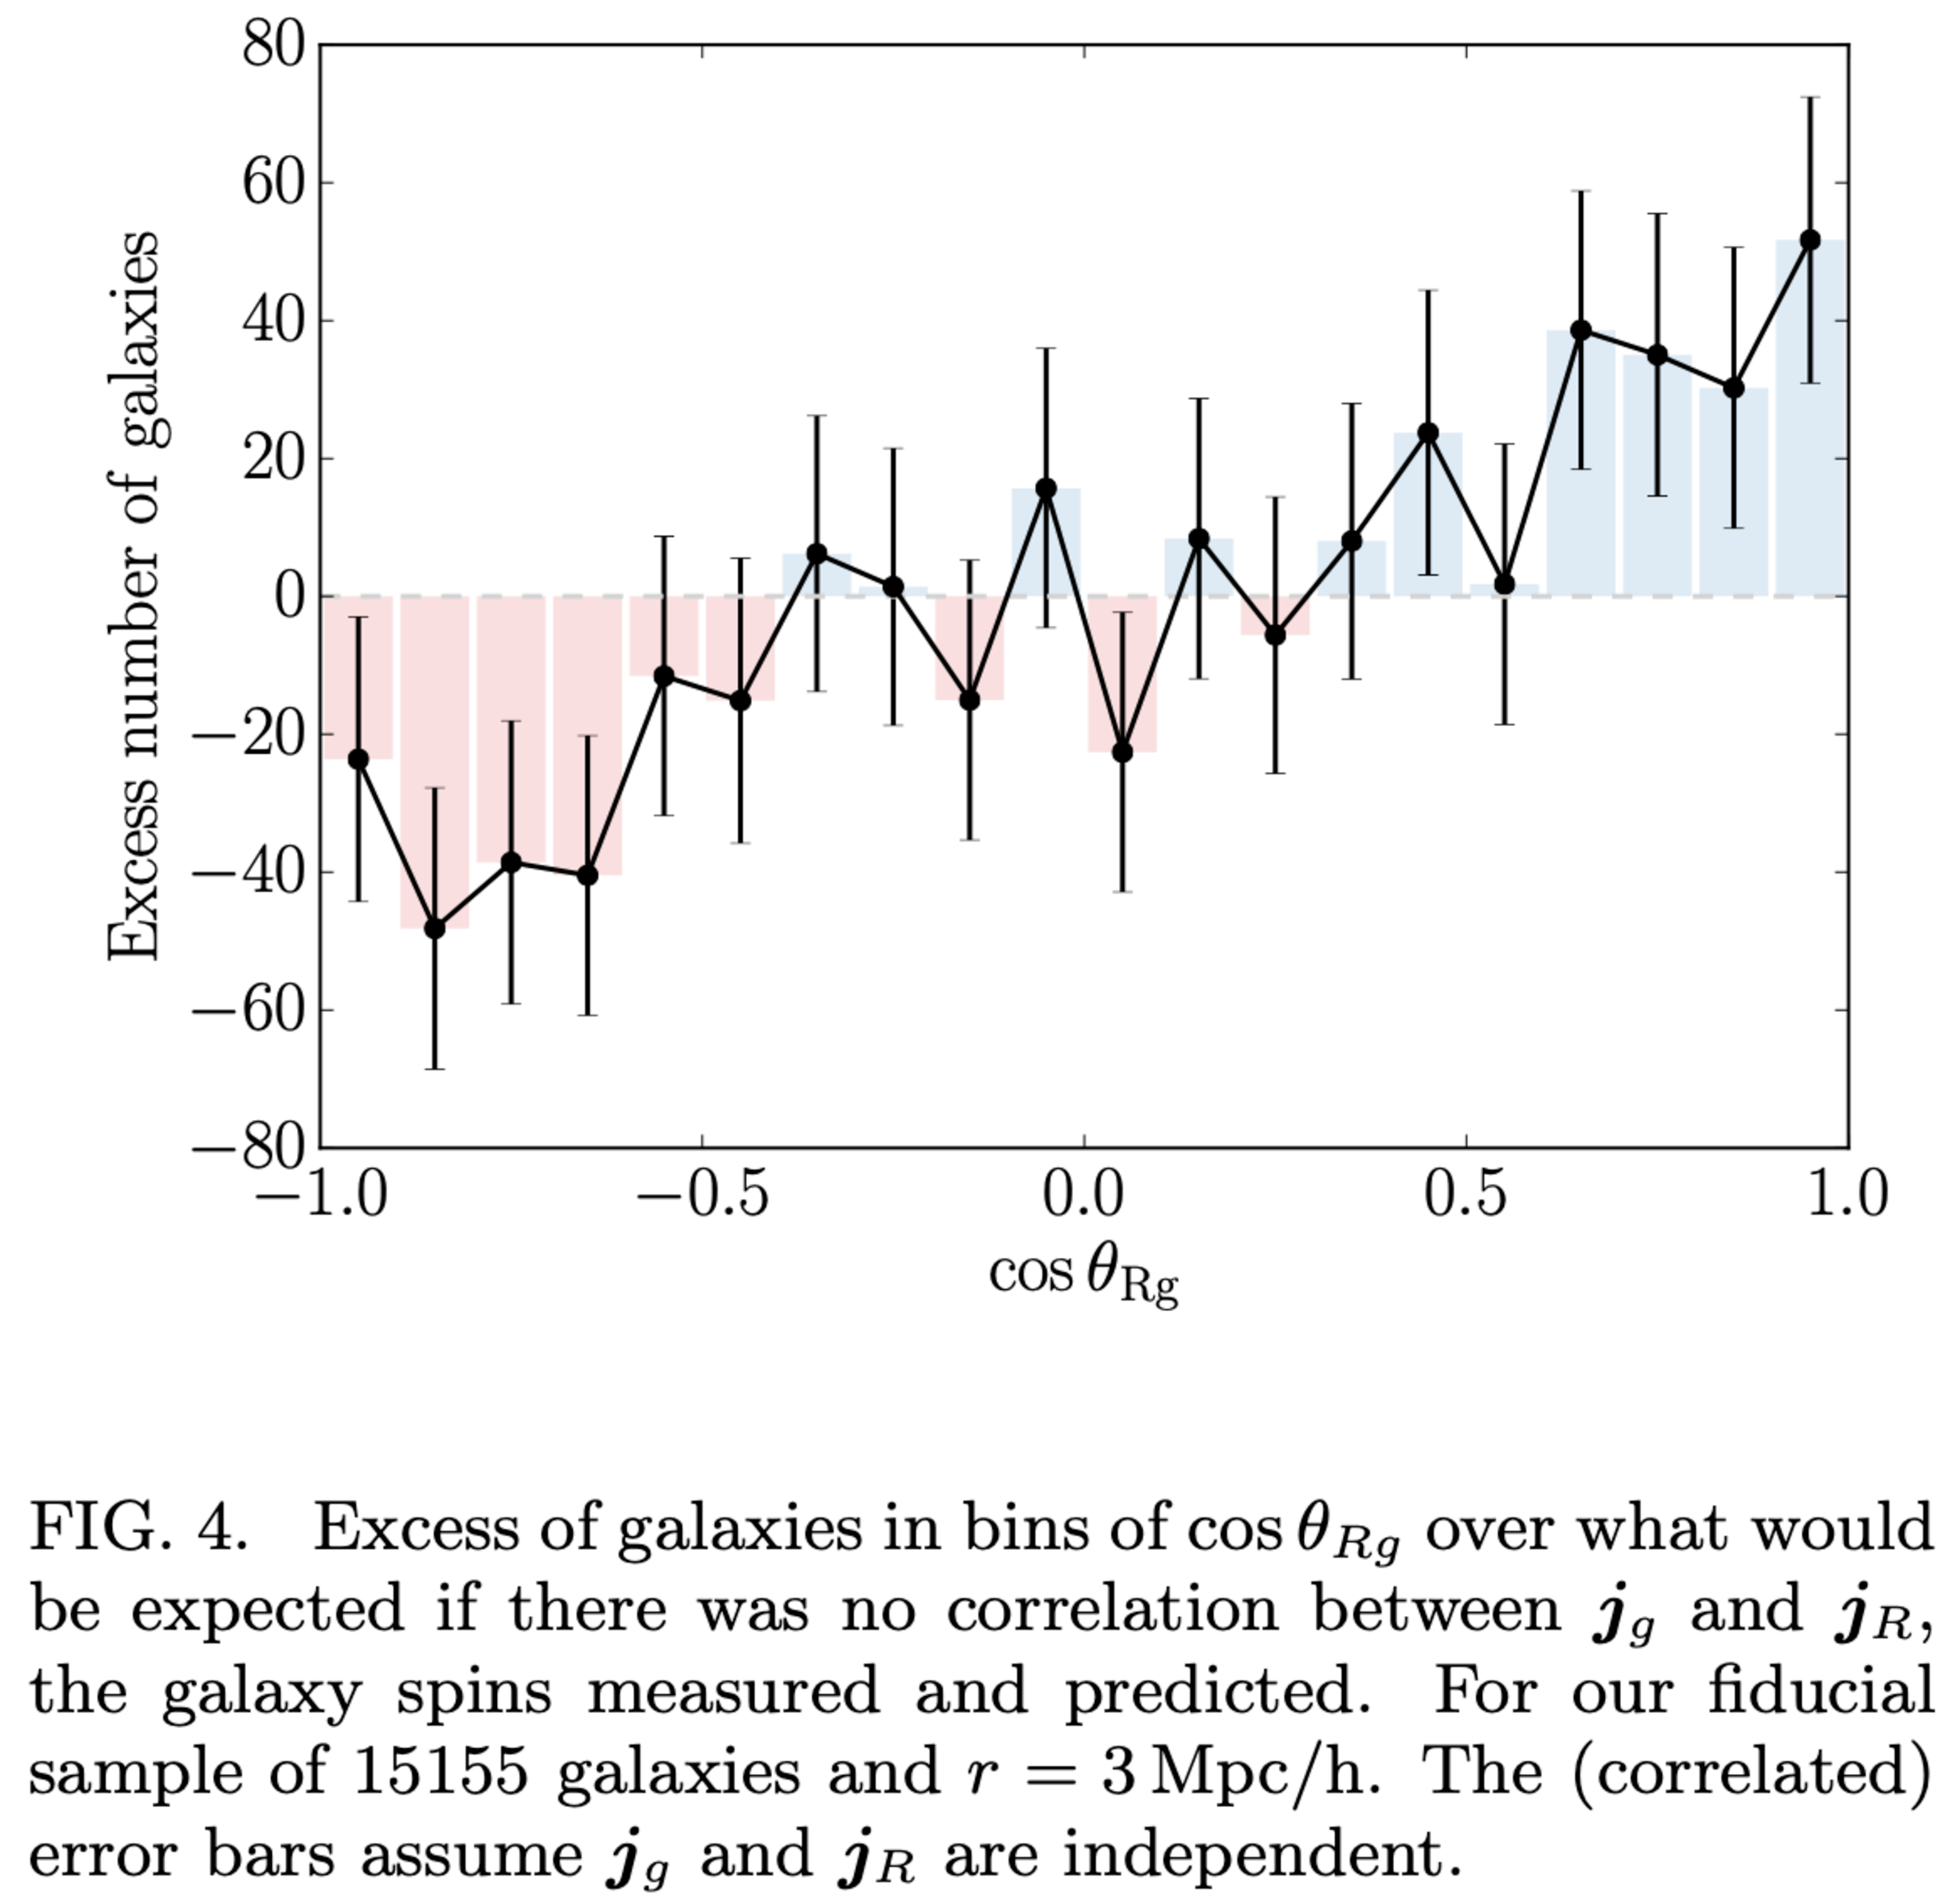
\includegraphics[width=2.9in]{Figures/spincorr.pdf}  
Motloch+ 2021
  }


  
\frame{
\vspace{-0.5in}
    \frametitle{Galaxy Spin Helicity}
    \begin{itemize}
    \item statistical isotropy and homogeneity allows for helicity asymmetry (e.g. weak force)
        \item NOT Goedel/Longo effect (``net $k$ independent left/right spin'')
        \item angular momentum measures twist of tidal tensor
        \item helicity measures twist projected along $k$ vector 
     \end{itemize}
  }

  \frame{
    \frametitle{Nature}
\vspace{-0.3in}\center{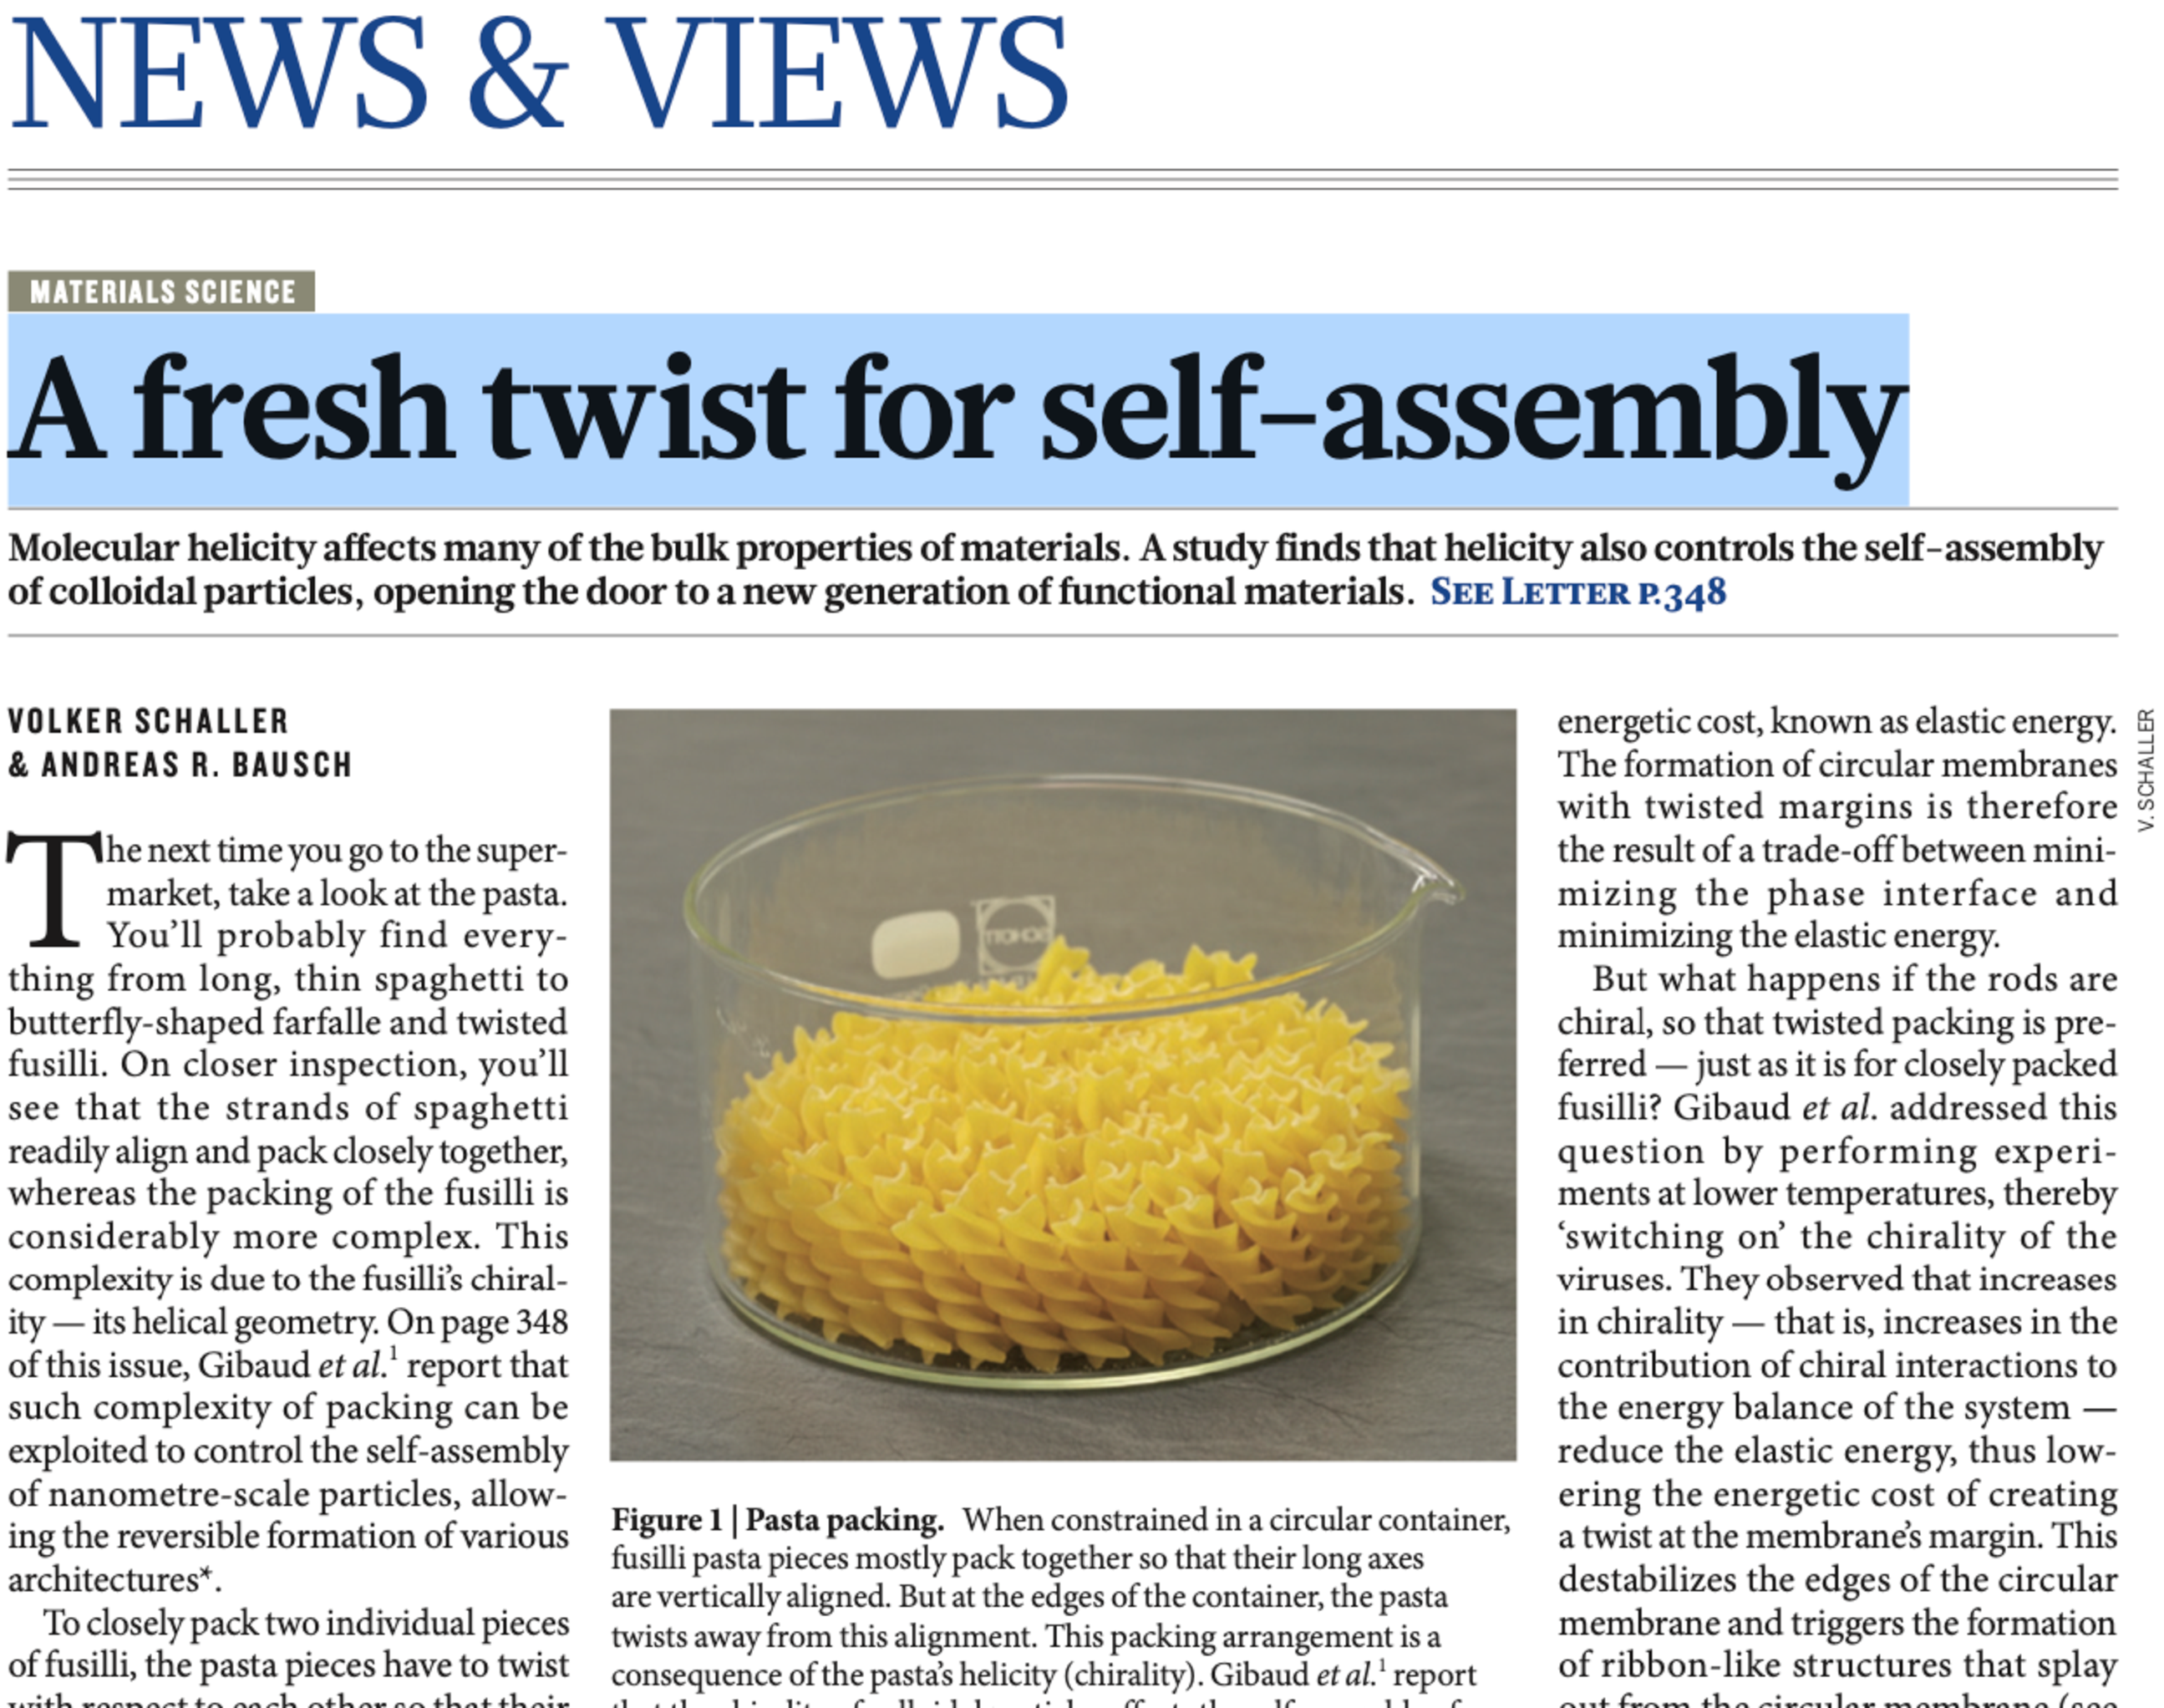
\includegraphics[width=4.0in]{Figures/twist.pdf}}
V Schaller \& A. Bausch 2012, Nature, 481, 268
}
  \frame{
    \frametitle{Pastarimeter}
    %\vspace{-0.3in}
    \center{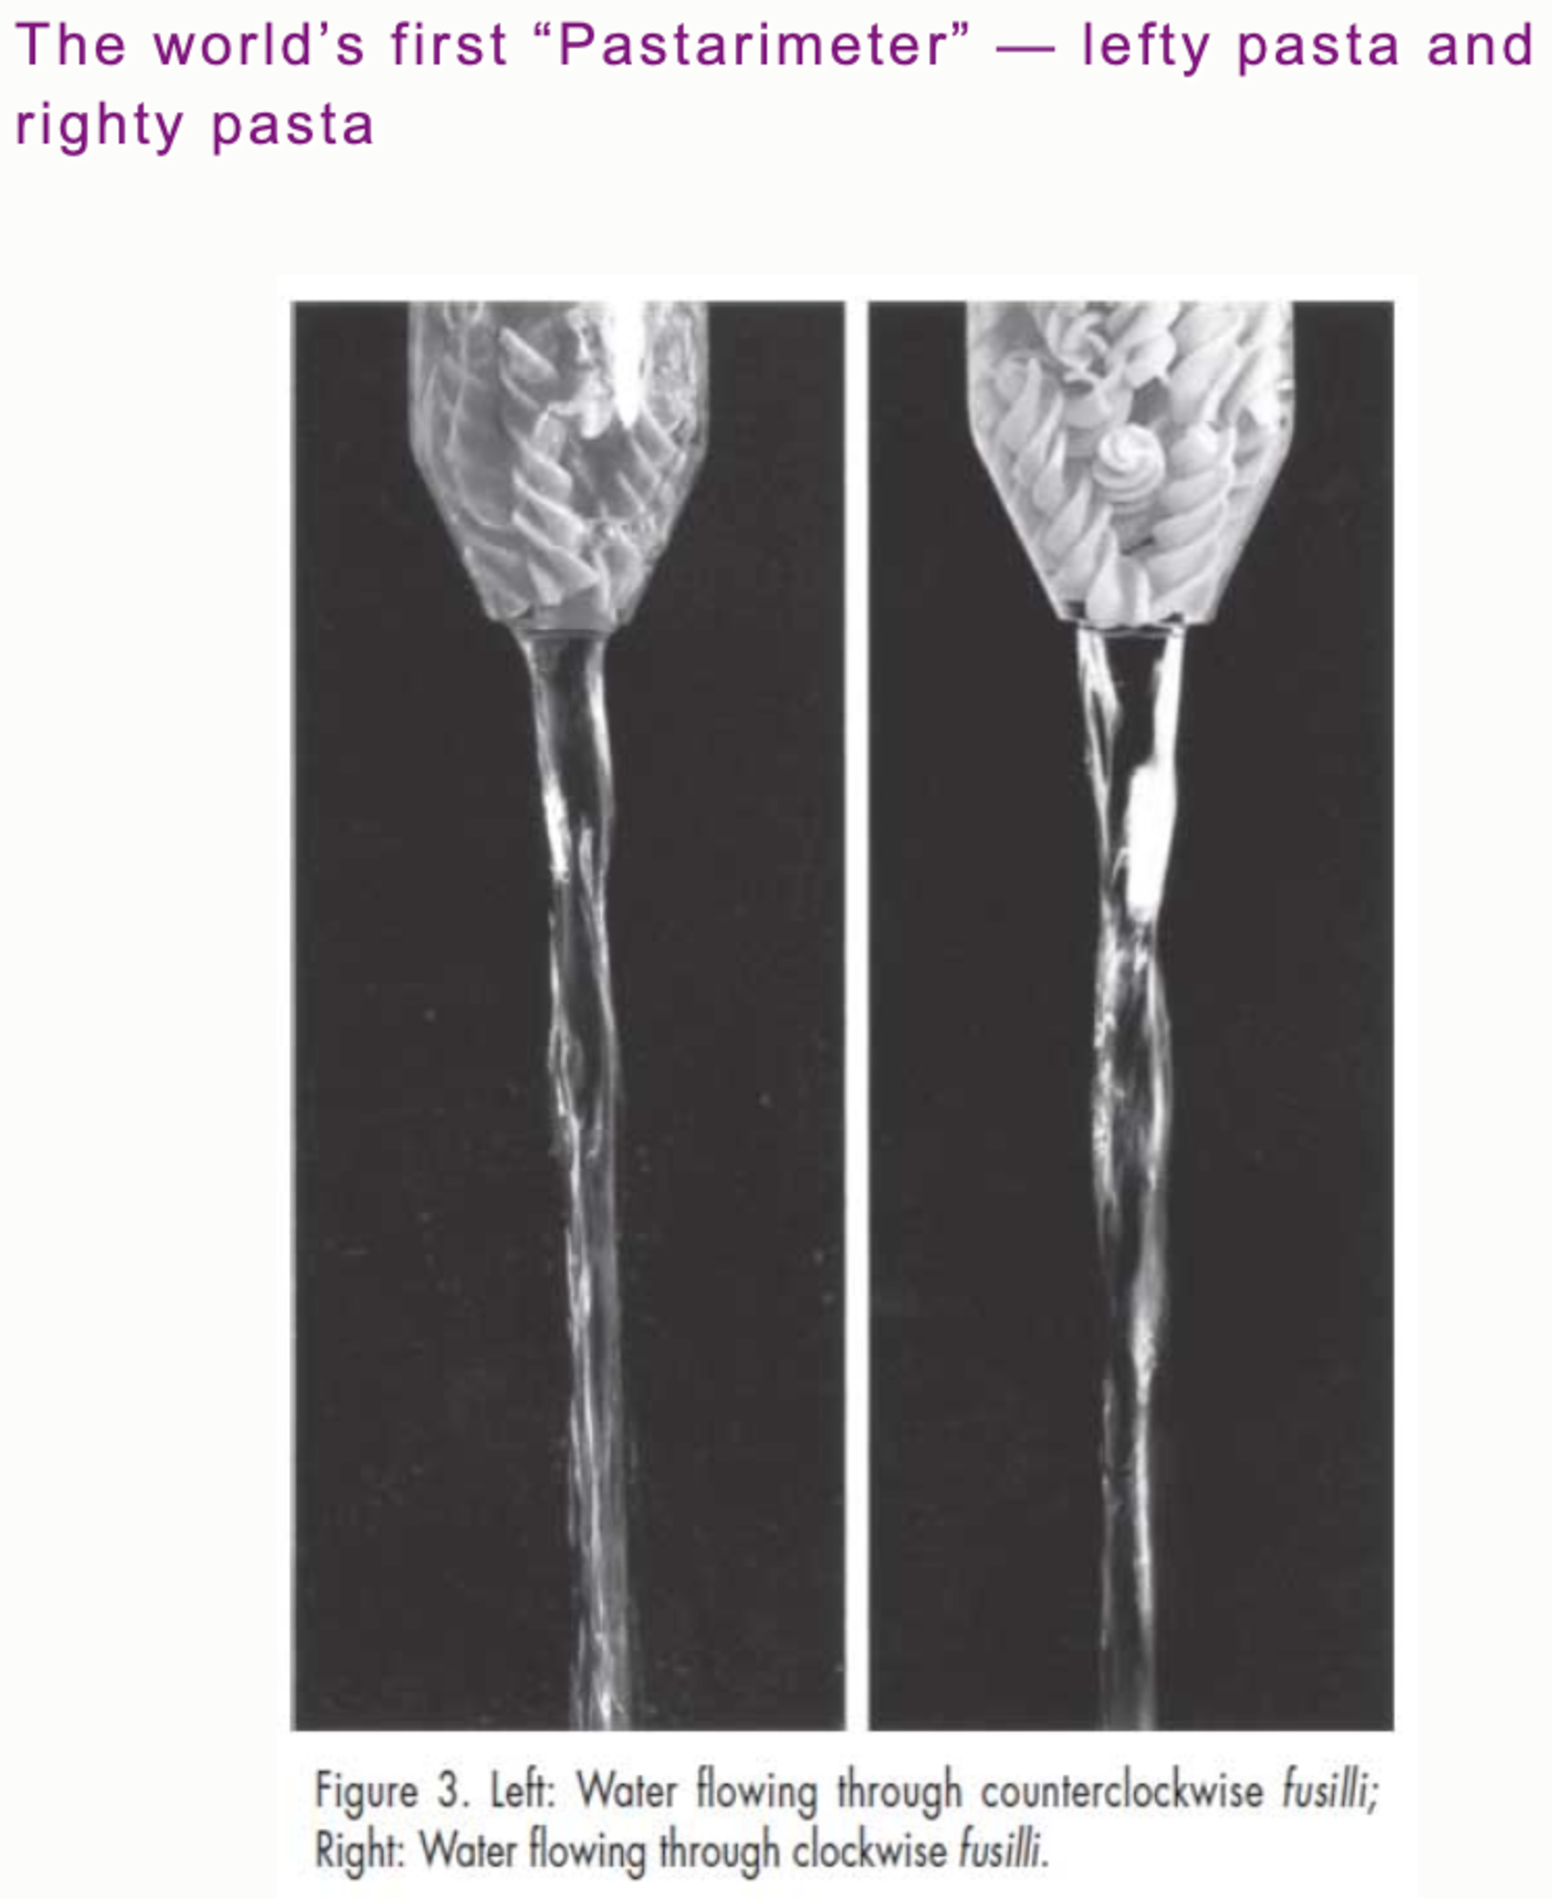
\includegraphics[width=2.5in]{Figures/pastarimeter.pdf}}
{\tiny Saxon et al 2002, J. Chem. Ed, 79, 1214}
}


 \frame{
    \frametitle{ELUCID projection}
    \begin{itemize}
    \item $J^\mathrm{IC}_a=  \epsilon_{abc}
\partial_{bk} \phi^r
\partial_{kc} \rho^r$
    \item  $\mathbb{P}^{L/R}_{ab}(\mathbf{k}) = 
  \frac{1}{2}
  \left[
  \(\delta_{ab} - \hat k_a \hat k_b\) 
  \pm    i \epsilon_{abc} \hat k_c \right] $
    \item   $\tilde J^\mathrm{IC}_{L/R,a}(\mathbf{k}) \equiv
  \mathbb{P}^{L/R}_{ab}(\mathbf{k}) 
  \tilde J^\mathrm{IC}_b(\mathbf{k})$
    \item  $\mu_X = \left\langle 
  \frac{\bs{J}^g}{|\bs{J}^g|}
  \cdot
  \frac{\bs{J}^\mathrm{IC}_X}{|\bs{J}^\mathrm{IC}_X|}
  \right\rangle \ \ \ \ \ X \in \{L, R\}$
\item $\mu_- = \mu_L - \mu_R$
     \end{itemize}
  }


  
\frame{
\vspace{-0.5in}
    \frametitle{Helicity results}
    \begin{itemize}
    \item   $\mu_L &=& \(0.41 \pm 0.53\) \times 10^{-2}$  maximal left is allowed
      \item $\mu_R &=& \(1.99 \pm 0.53\) \times 10^{-2} $  maximal right is disfavoured!
      \item $\mu_- = \(-1.58 \pm 0.75\) \times 10^{-2}$  Parity symmetry is allowed \dSmiley % \DejaSans{ ☺}
     \end{itemize}
  }

  
\frame{
\vspace{-0.5in}
    \frametitle{Conclusions}
    \begin{itemize}
      \item helicity is a preserved non-Gaussianity not contaminated
        by late time non-linearity
      \item claimed odd detections in LSS on large scales, upper
        bounds on helicity for  small scales.
      \item tidal classification of helical non-Gaussianity: vector,
        tensor
      \item reported excess in parity odd power not necessarily due to
        helicity, more work needed        
      \item B-mode (V,T, odd) non-Gaussianity not necessarily clean
      \item well preserved in galaxy spin, needs numerical work to
        quantify for other forms
     \end{itemize}
  }


\end{document}
